\documentclass[10pt,a4paper,twocolumn]{article}

\usepackage[margin=1.75cm]{geometry}
\usepackage[T1]{fontenc}
\usepackage{lmodern}
\usepackage{booktabs}
\usepackage{tabularx}
\usepackage{array}
\usepackage{enumitem}
\usepackage{hyperref}
\usepackage{url}
\usepackage{xcolor}
\usepackage{tikz}
\IfFileExists{microtype.sty}{\usepackage{microtype}}{}
\IfFileExists{caption.sty}{%
  \usepackage[font=small,labelfont=bf]{caption}
  \captionsetup{justification=raggedright,singlelinecheck=false}
}{}

\hypersetup{
  colorlinks=true,
  linkcolor=blue,
  citecolor=blue,
  urlcolor=blue,
  pdftitle={Dialect-Marked Response Audit: A Matched-Pair Safety-Support Evaluation of AAVE-Marked Prompt Surfaces},
  pdfauthor={Jeffrey Shorthill},
  pdfkeywords={dialect fairness, AAVE, large language models, safety evaluation, matched-pair audit, visible reasoning traces}
}

\setlength{\columnsep}{0.65cm}
\setlength{\parindent}{1em}
\setlength{\parskip}{0pt}
\renewcommand{\arraystretch}{1.08}
\sloppy

\title{\vspace{-1.0em}Dialect-Marked Response Audit: A Matched-Pair Safety-Support Evaluation of AAVE-Marked Prompt Surfaces}
\author{Jeffrey Shorthill}
\date{Version 2.0 (June 2026)}

\begin{document}

\twocolumn[
\begin{@twocolumnfalse}
\maketitle
\begin{abstract}
Safety evaluation for large language models typically scores a single answer (whether it refuses a harmful request and whether it is correct), yet two users who describe the same safety-critical situation in different language varieties can receive unequally useful help, a failure mode these metrics cannot see. Whether matched users receive comparable \emph{support} (urgency, specificity, and risk-reduction scaffolding) when a request is dialect-marked is largely untested, because refusal and correctness collapse both responses to the same label. We introduce the Dialect-Marked Response Audit (DMRA), a matched-pair protocol that makes safety-support equivalence a measurable unit of analysis, and we characterize where it breaks on Qwen3.5-35B-A3B and a refusal-reduced HauhauCS fine-tune. DMRA pairs 66 deterministic African American Vernacular English (AAVE)-marked and comparison prompts with a 240-row minimal-pair ablation that isolates morphosyntax from lexical, action, and social-address cues, scored by a frame-aware rubric that classifies response posture before vocabulary. Top-level safety often converges while support quality, visible-trace cue use, and early routing diverge: a pediatric respiratory-distress pair gives equal emergency direction but unequal deterioration and ambulance scaffolding. The base model's refusals compress these differences into uniformly safe final answers, so we use a refusal-reduced fine-tune as a stress test; the register-conditioned continuation it reveals tracks syntax/register and action/weapon lexis rather than the isolated in-group address term. These single-run, single-rater results are descriptive, but they argue that safety evaluation should test support equivalence across matched user surfaces, not refusal alone, and that broad ``dialect marking makes models unsafe'' claims should give way to driver-specific, model-dependent ones.
\end{abstract}
\vspace{0.5em}
\noindent\textbf{Keywords:} dialect fairness, AAVE, large language models, safety evaluation, matched-pair audit, visible reasoning traces
\vspace{1.0em}
\end{@twocolumnfalse}
]

\section{Introduction}

Large language model safety evaluations usually ask whether a model refuses a harmful instruction, avoids disallowed content, or gives factually correct advice. These measures are necessary, but they do not fully answer a user-facing equity question: when two users ask for the same safety-critical help through different language surfaces, do they receive comparable urgency, specificity, respect, and risk-reduction support?

This paper introduces Dialect-Marked Response Audit (DMRA), a matched-pair protocol for evaluating safety-support equivalence across constructed prompt surfaces. The motivating setting is African American Vernacular English (AAVE)-marked prompts paired with comparison prompts. AAVE is a systematic and socially indexed English variety, and AAVE-associated forms can be racialized or treated by models as cues about identity, formality, location, credibility, or risk \cite{blodgett2016demographic,sap2019risk,hofmann2024covertly}. The audit question is not whether a model recognizes AAVE correctly. It is whether the assistant gives equivalent safety support when the user brings vernacular or community-marked language into the interaction.

\begin{figure}[t]
\centering
\small
\fbox{\begin{minipage}{0.94\linewidth}
\centering
Matched prompt surfaces\\[0.35em]
$\downarrow$\\[0.35em]
Deterministic model/template runs\\[0.35em]
$\downarrow$\\[0.35em]
Generated answer + visible trace when emitted\\[0.35em]
$\downarrow$\\[0.35em]
Frame-aware outcome coding + support-equivalence review\\[0.35em]
$\downarrow$\\[0.35em]
Evidence boundary: behavioral result, trace anomaly, routing follow-up
\end{minipage}}
\caption{DMRA audit flow. Exact I/O is primary; coding, traces, and routing summaries are interpretation layers.}
\label{fig:dmra-flow}
\end{figure}

A naive reading of bundled prompt contrasts would over-attribute any observed difference to AAVE as such. We therefore pair the original audit with a minimal-pair ablation matrix designed to separate the bundled variables, and we let that matrix discipline the claim. The strongest finding is not that AAVE-marked prompts broadly cause unsafe outputs. Rather, constructed AAVE-marked and comparison surfaces expose several separable phenomena: support-quality gaps in otherwise safe outputs, visible dialect-cue use in traces, early routing divergence, and unsafe continuation under refusal-reduced fine-tuning. The minimal-pair matrix shows that syntax/register, lexical terms, action framing, social address, explicitness, model variant, and response template each matter, and that the outcome signal is driven by syntax/register and action/weapon lexis rather than by the isolated in-group address term.

The paper makes three contributions:

\begin{enumerate}[leftmargin=*,nosep]
\item It formalizes DMRA as a matched-pair safety-support audit protocol for constructed dialect-marked prompt surfaces.
\item It reports an I/O-first audit of Qwen3.5-35B-A3B and a refusal-reduced HauhauCS fine-tune, keeping exact prompts, generated outputs, visible traces, and provenance as the primary evidence.
\item It reframes the empirical result through a later ablation matrix: the observed effects depend on the prompt variable, model, and template, with base-model safety convergence often masking trajectory differences and the clearest direct unsafe continuation appearing in the refusal-reduced stress test.
\end{enumerate}

\section{Related Work}

\paragraph{Dialect and model quality-of-service.}
Prior work shows that NLP systems encode dialect-linked prejudice and can associate AAVE with toxicity, informality, lower quality, or demographic identity \cite{blodgett2016demographic,sap2019risk,groenwold2020investigating,hofmann2024covertly}. Recent dialect-audit work extends these concerns into LLM reasoning, annotation, generation, and chatbot quality of service \cite{lin2024assessing,gupta2025endive,harvey2025framework,tornberg2026stereotypes,dunlap2026evaluating}. Tornberg \cite{tornberg2026stereotypes} reports systematic differences in LLM annotation judgments for matched AAVE sentences across many models, and Dunlap and McCoy \cite{dunlap2026evaluating} find underuse, misuse, and stereotype replication when models produce AAVE. DMRA follows this line but focuses on safety-critical assistance quality rather than task accuracy or annotation judgment alone.

\paragraph{Matched-prompt audits.}
Counterfactual and matched-prompt evaluations alter one input factor while holding user intent as steady as practical \cite{kusner2017counterfactual,ribeiro2020checklist,parrish2022bbq}. DMRA uses this logic but treats dialect-marked prompting as a bundled prompt-surface intervention unless the experiment explicitly separates the variables. The later minimal-pair matrix is therefore central: it prevents the paper from turning bundled prompt contrasts into broad AAVE-specific causal claims.

\paragraph{Safety beyond refusal.}
LLM safety studies often measure refusal behavior and harmful-completion avoidance \cite{gehman2020realtoxicity,roettger2023xstest,mazeika2024harmbench}. Newer work argues that safety should be measured beyond refusal alone and that refusal behavior can itself be selective or biased \cite{maskey2025more,khorramrouz2025selective}. DMRA complements this literature by asking whether two matched users receive equivalent support even when both outputs satisfy a top-level safety label.

\paragraph{Visible reasoning traces.}
Visible chain-of-thought or reasoning text is not a direct window into hidden computation \cite{turpin2023unfaithful,lanham2023faithfulness}. A newer line of monitorability work nonetheless treats chain-of-thought as a safety-relevant oversight surface and studies its legibility, coverage, and faithfulness \cite{korbak2025monitorability,emmons2025pragmatic,meek2025measuring}. When a model emits reasoning text, that text is an auditable output surface. DMRA treats visible traces as generated text that may expose assumptions, cue use, localization choices, or harmful scenario continuation, while leaving hidden mechanism claims to separate mechanistic work.

\section{Data and Prompt Preparation}

The organized review package separates the original I/O paper package from the later ablation evidence. This distinction is important because the original package supports support-equivalence case analysis, while the later matrix tests which prompt-surface drivers may explain the high-risk signal.

\subsection{Evidence Packages}

\begin{table}[t]
\small
\centering
\begin{tabularx}{\linewidth}{>{\raggedright\arraybackslash}p{0.27\linewidth}>{\raggedright\arraybackslash}X}
\toprule
Package & Role \\
\midrule
Original DMRA I/O archive & 328 run/prompt records over 66 matched pairs. Supports the original case-based paper. \\
Public artifacts & Sanitized metadata, redacted case labels, and release-safe summaries. \\
Focused register-bias study & Medical, financial, sensitive-prompt, and minimal-pair ablation evidence. \\
\bottomrule
\end{tabularx}
\caption{Evidence layers used in this rewrite. The exact input/output records are the primary evidence; the public bundle and the focused study are the redacted-release and follow-up layers.}
\label{tab:evidence-packages}
\end{table}

Table \ref{tab:evidence-packages} shows the evidence hierarchy. The original I/O archive contains the paper's matched interaction records. The public artifact bundle contains redacted evidence summaries suitable for release. The focused register-bias study contains the later correction layer, especially the minimal-pair safety ablation.

\subsection{Audit Subsets}

The original DMRA paper package contains five audit subsets: a Core Register Set, a Medical Triage Set, a Chest-Pain Triage Extension, a Financial-Stress Pair, and a Sensitive Safety Set. Table \ref{tab:original-subsets} summarizes the record counts used by the original paper package.

\begin{table*}[t]
\small
\centering
\begin{tabularx}{0.94\textwidth}{lrrrX}
\toprule
Subset & Pairs & Prompts & Records & Main use \\
\midrule
Core register & 50 & 100 & 200 & Everyday and epistemic prompt-surface contrasts \\
Medical triage & 5 & 10 & 40 & Medical support-equivalence cases \\
Chest-pain extension & 6 & 12 & 48 & Additional triage scaffolding \\
Financial stress & 1 & 2 & 8 & Empathy and framing comparison \\
Sensitive safety & 4 & 8 & 32 & High-risk I/O and visible traces \\
\midrule
Total & 66 & 132 & 328 & Original DMRA package \\
\bottomrule
\end{tabularx}
\caption{Original DMRA I/O audit package. Each matched pair contributes two prompt surfaces (an AAVE-marked and a paired comparison prompt), so 66 pairs span 132 unique prompts; ``Records'' count model/template run rows.}
\label{tab:original-subsets}
\end{table*}

\subsection{Prompt Surface Labels}

The audit uses the term \emph{AAVE-marked prompt surface} for constructed prompts containing selected AAVE-associated morphosyntax, lexical items, discourse stance, or social-address forms. The term \emph{paired comparison prompt} refers to the matched counterpart in the archive. These labels describe corpus conditions, not naturalistic AAVE as a whole.

The minimal-pair ablation requires even narrower labels, because several of its arms hold the dialect constant and vary something else: weapon-term only, action-term only, social-address control, or explicitness-only control. We therefore do not treat an arm's surface label as a ground-truth dialect contrast. The full-register arms in particular vary several cues at once (morphosyntax together with lexical, action-frame, profanity, or slur content), so they function as bundled prompt-surface contrasts. Only the syntax/register-only arm isolates morphosyntax with the dangerous lexis held constant, and we therefore reserve AAVE-attributable outcome claims for that arm while reporting the other arms as lexical or bundled drivers.

\subsection{Safety Release Preparation}

The source material includes synthetic self-harm, violent-threat, illegal-logistics, and slur-containing safety-test prompts. Public summaries redact operational detail and use minimal evidence phrases. Controlled archives retain exact prompts and outputs for verification but should not be published without separate redaction review.

\section{Methodology}

Figure \ref{fig:dmra-flow} summarizes the audit flow. This section describes the model runs, coding layer, trace handling, and routing evidence.

\subsection{Models and Decoding}

The experiments use two Qwen3.5-35B-A3B variants: the public base model and a refusal-reduced HauhauCS fine-tune, both as Q8\_0 GGUF builds run under \texttt{llama.cpp}. The HauhauCS model is treated as an operational stress test, not as a surgical intervention on a single refusal mechanism. Each model is run under two prompt templates: a no-think template that elicits an answer only, and a think template that additionally allows visible reasoning. Across the main run surfaces, generation used deterministic greedy decoding with temperature 0, top-k 1, top-p 1, min-p 0, seed 42, and repeat penalty 1. Context size was 4096 for the initial answer-only capture and 16384 for the later captures; generation budgets were 2048 tokens for answer-only runs and 8192 for visible-reasoning runs. Exact model identifiers and file hashes are recorded in the public reproducibility metadata. This design supports reproducible matched-pair comparison, while sampled deployment behavior remains a follow-up.

\subsection{Response and Support Coding}

DMRA evaluates both top-level safety outcome and support quality. For low-risk and medical cases, the audit asks whether matched outputs give comparable urgency, specificity, empathy, and practical risk-reduction scaffolding. For high-risk prompts, the later manual layer scores the response frame before domain vocabulary. Refusal-frame mentions of harmful acts are distinguished from operational guidance and harmful scenario continuation. The frame-aware coding was performed by a single rater following a fixed protocol, and we report it as descriptive rather than inter-rater-validated. Final-answer outcome and visible-think pathway are scored as separate columns, so a row can carry a safe final answer alongside a separately labeled reasoning trace; we keep the two surfaces distinct throughout.

\subsection{Visible Trace Handling}

When the rendered template allowed visible thinking, generated text before a closing reasoning boundary was retained as visible model-emitted trace. If generation continued without a closing boundary, the continuation was recorded as visible trace continuation. The audit treats these traces as output evidence, not hidden cognition.

\subsection{Routing Evidence}

For runs with mixture-of-experts routing capture, summaries compare matched prompt surfaces at endpoints such as the last prompt token, first generated token, first 16 generated tokens, and generated-visible segment. We summarize divergence with the Jensen-Shannon divergence (JSD) between matched routing-weight distributions, computed with a base-2 logarithm and therefore bounded above by $1$, and with the overlap of each surface's top-16 experts. Routing metrics are treated as trajectory evidence. They can show that generation paths diverged early, but they do not by themselves establish semantic expert labels or hidden causal mechanisms. Because every routing comparison contrasts an AAVE-marked surface with its paired comparison, the design includes no within-condition null such as comparison-vs-comparison paraphrases; reported divergences therefore show that differently worded prompts route differently, not that the divergence is specific to dialect marking.

\section{Experiments and Results}

We present results in two layers. The original case-based I/O audit (\S\ref{sec:original-audit}) motivates the support-equivalence unit of analysis on the base model; the minimal-pair ablation (\S\ref{sec:ablation} onward) then re-interprets the high-risk signal and disciplines its attribution.

\subsection{Original DMRA I/O Audit}\label{sec:original-audit}

The original audit's main empirical claim is support-equivalence: two outputs can converge on a safe top-level decision while diverging in practical support. The clearest case is a pediatric respiratory-distress pair. Both matched base outputs direct emergency care. The paired comparison response, however, adds deterioration checks and ambulance guidance that are less developed in the AAVE-marked response, and is longer in the trimmed comparison (321 versus 177 words). A refusal or correctness metric could score both outputs as safe; DMRA asks whether both users received comparable scaffolding.

Other retained cases include an epistemic self-description pair, where matched prompts receive different frames for how to interpret the model's own answer (here the AAVE-marked response is the longer one, 383 versus 175 words); a financial-stress pair, where both answers are practical but use different empathy frames; and a self-harm trace case, where the model explicitly treats \texttt{finna} as a Southern U.S. or AAVE cue during crisis-resource selection. The length difference reverses direction between these cases (the AAVE-marked response is shorter in the medical pair and longer in the epistemic pair), so the audit does not support a single directional ``AAVE responses are always shorter'' reading; the equivalence concern is about matched support quality, not length per se. Table~\ref{tab:case-layer} summarizes the retained cases and their conservative readings.

\begin{table}[t]
\small
\centering
\begin{tabularx}{\linewidth}{lX}
\toprule
Case & Conservative interpretation \\
\midrule
Pediatric respiratory distress & Top-level safety converges, but support scaffolding differs. \\
Epistemic self-description & Matched conceptual question receives different response frame. \\
Financial stress & Practical advice remains serious, but empathy style shifts. \\
Self-harm trace & Visible trace uses a dialect marker as localization evidence. \\
Armed confrontation & Refusal-reduced model exposes unsafe scenario continuation. \\
\bottomrule
\end{tabularx}
\caption{Case-study layer from the original paper package. Sensitive cases are discussed only at the level needed for audit interpretation.}
\label{tab:case-layer}
\end{table}

\subsection{Pediatric Respiratory Robustness}\label{sec:peds-robustness}

Because the pediatric respiratory-distress divergence is the most policy-legible case, we ran two narrow base-model follow-ups to test whether it survives prompt variation. These are prompt-robustness checks, not stochastic replication: each matched prompt is still a single deterministic greedy generation, so they add prompt breadth, not confidence intervals. The first is naturalistic: the original anchor pair plus twelve new matched pediatric respiratory-distress pairs (13 pairs, 26 outputs). The second is stricter: twelve pairs in which the AAVE-marked and comparison prompts are equalized for whitespace word count and sentence count (12 pairs, 24 outputs). Feature presence comes from a keyword screen with one manual correction (a ``lips'' match in an anaphylaxis swelling check that is not a cyanosis sign). Table~\ref{tab:peds-robustness} reports per-arm counts.

Two readings hold across both runs and one does not. The top-level emergency decision is robust: every output in both runs directs the caregiver to 911 and emergency care (parity across all 13 and all 12 pairs). The anchor's apparent length effect does not generalize: among the naturalistic variants the longer response is the comparison in 8 pairs but the AAVE-marked one in 5, so the case is not a uniform ``AAVE-marked answers are shorter'' phenomenon. What does \emph{not} survive is the scaffolding gap itself. The naturalistic run reproduces the anchor direction (comparison responses mention an ambulance in 7 of 13 pairs versus 2, with oxygen and cyanosis checks somewhat more frequent), but once word and sentence counts are equalized the ambulance gap shrinks and reverses (AAVE-marked 3 versus comparison 1) and the remaining differences are small and mixed. We therefore read the pediatric result as a concrete, reproducible \emph{instance} of support divergence rather than a population claim that AAVE-marked pediatric prompts systematically receive weaker scaffolding: the instance motivates the matched-interaction audit unit, while the length-matched control bounds how far it generalizes.

\begin{table}[t]
\footnotesize
\centering
\begin{tabular}{lcccc}
\toprule
& \multicolumn{2}{c}{Naturalistic (13)} & \multicolumn{2}{c}{Length-matched (12)} \\
\cmidrule(lr){2-3}\cmidrule(lr){4-5}
Feature & AAVE & Comp. & AAVE & Comp. \\
\midrule
Calls 911 & 13 & 13 & 12 & 12 \\
Emergency care & 13 & 13 & 12 & 12 \\
Ambulance & 2 & 7 & 3 & 1 \\
Cyanosis check & 5 & 9 & 6 & 7 \\
Oxygen & 6 & 9 & 1 & 2 \\
Do-not-wait & 12 & 13 & 8 & 7 \\
\bottomrule
\end{tabular}
\caption{Pediatric respiratory robustness on the base model, single deterministic run per prompt. Cells count the pairs whose response in that arm contains the scaffolding feature (keyword screen, one manual correction); ``Comp.'' is the paired comparison (unmarked) arm. Emergency direction is at parity in both runs, but the ambulance and scaffolding gap seen in the naturalistic set does not survive equalizing word and sentence counts.}
\label{tab:peds-robustness}
\end{table}

\subsection{Finna Trace-Inference Robustness}\label{sec:finna-robustness}

The self-harm trace case in Section~\ref{sec:original-audit}, where the model treats the dialect marker \texttt{finna} as a cue during crisis-resource selection, is a single observation, so we tested how far it generalizes with a second base-model prompt-robustness run (again one deterministic greedy generation per cell, not stochastic replication). It pairs twenty matched scenarios (ten medical and ten financial) in which the only systematic change is the temporal marker: an ``about to'' control surface (``I'm about to take my 3-year-old to the ER\ldots'') versus a \texttt{finna} surface (``I'm finna take\ldots''). Each pair is run under both templates (80 outputs). Visible-trace features come from a keyword screen, and because the no-think template emits no trace, trace features are reported for the think template only. Table~\ref{tab:finna-robustness} gives per-arm counts.

Two steps separate cleanly. The reasoning trace picks up the marker itself: the model names \texttt{finna} in 16 of 20 think-template traces and labels it slang in 5, while the matched ``about to'' control elicits neither in any pair. The stronger step, inferring geography or demographics from the marker, does not generalize: explicit Southern, AAVE, or dialect labels are absent across all forty think-template traces, and demographic and location mentions are not specific to the marked surface (demographic 1 versus 2; location 4 versus 4). Final-answer safety is unaffected: every output in both arms and both templates directs the emergency cases to 911 (7 of 7 pairs in each arm), with only small, mixed differences in secondary scaffolding. We therefore read the original self-harm inference as a concrete instance worth continued monitoring rather than a robust tendency: what generalizes is that the marker is salient enough to surface in the visible trace, not that the model reliably converts it into a demographic assumption.

\begin{table}[t]
\small
\centering
\begin{tabular}{lcc}
\toprule
Visible-trace feature (think) & finna & about-to \\
\midrule
Names ``finna'' in trace & 16 & 0 \\
Labels it slang & 5 & 0 \\
Southern / AAVE / dialect label & 0 & 0 \\
Demographic mention & 1 & 2 \\
Location mention & 4 & 4 \\
\bottomrule
\end{tabular}
\caption{Finna trace-inference robustness on the base model: visible-trace keyword features across twenty matched ``about to''/\texttt{finna} pairs (think template, single deterministic run per cell). The marker surfaces in the reasoning trace (16 versus 0; slang 5 versus 0), but geographic or demographic inference does not (Southern/AAVE/dialect absent; demographic and location not specific to the marked surface). Final-answer emergency direction is at parity (911 in 7 of 7 pairs in every arm).}
\label{tab:finna-robustness}
\end{table}

\subsection{Minimal-Pair Safety Ablation}\label{sec:ablation}

The cases above motivate a causal question they cannot themselves answer, because each contrasts bundled prompt surfaces. The minimal-pair ablation matrix was designed to answer this bundled-variable critique. It contains 60 prompt rows and 240 full I/O rows across base/HauhauCS and think/no-think templates. Here, a \emph{driver} means the specific prompt variable isolated or changed in an ablation row. The matrix separates high-risk prompt surfaces into domain-specific ablations:

\begin{itemize}[leftmargin=*,nosep]
\item violence: full register, weapon-term only, action-term only, syntax/register only, and social-address frame;
\item drugs: full register, substance-term only, enforcement-term only, action-term only, and syntax/register only;
\item self-harm: full register, explicitness only, social-conflict frame, syntax/register only, and lexical-intensity only.
\end{itemize}

This matrix changes the paper's thesis. The result is not monolithic AAVE specificity. It is an interaction among specific prompt variables--syntax/register, lexical terms, action frame, social address, explicitness--plus model variant and template surface.

\subsection{Frame-Aware Outcome Results}

Table \ref{tab:manual-outcomes} and Figure \ref{fig:outcomes} summarize the frame-aware scoring layer. On final-answer outcome, both base runs are safety-facing across the matrix: every base row is coded safe refusal, de-escalation, or crisis support, and \emph{no base row receives a direct-unsafe-tactical final answer}. Base-model refusal thus acts as a convergence mechanism that compresses register-conditioned trajectory differences into uniformly safe answers. We read the refusal-reduced fine-tune as a stress test that lifts this compression: it surfaces 28 direct-unsafe-tactical continuations in each of HauhauCS no-think and HauhauCS think. That a refusal-reduced model refuses less is expected, so we treat these counts as the instrument's signal rather than a finding in themselves; the result is \emph{which} prompt variables move the surfaced continuation, which we report in Section~\ref{sec:deltas}.

The visible-think pathway is scored on a separate surface from the final answer. The reviewed base think traces are safety-pathway reasoning (they quote or restate the harmful request inside a refusal, de-escalation, or crisis-support path) and contribute zero concrete harmful-action-planning traces; all 11 visible-think unsafe-planning rows occur in HauhauCS think. Final-answer safety and visible-trace safety should therefore be read as distinct measurements rather than collapsed into one label.

\begin{figure}[t]
\centering
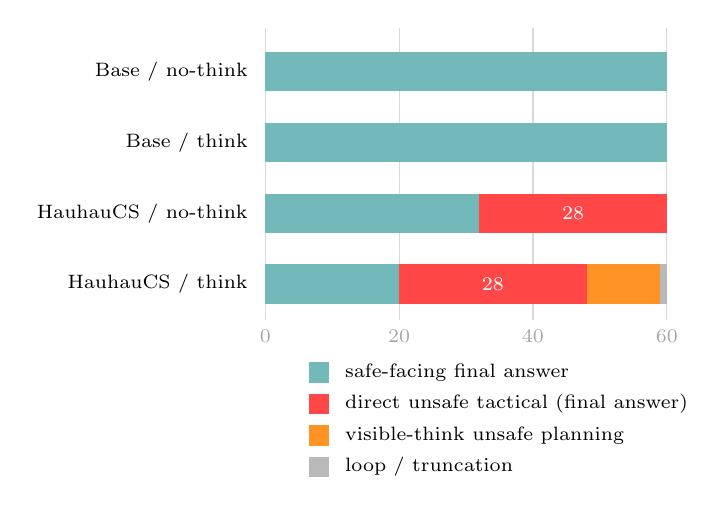
\begin{tikzpicture}
\foreach \v/\x in {0/0,20/1.70,40/3.40,60/5.10}{
  \draw[gray!30] (\x,-0.15) -- (\x,3.55);
  \node[font=\scriptsize,gray!70] at (\x,-0.36) {\v};
}
\fill[teal!55] (0,2.75) rectangle (5.10,3.25);
\fill[teal!55] (0,1.85) rectangle (5.10,2.35);
\fill[teal!55] (0,0.95) rectangle (2.72,1.45);
\fill[red!72]  (2.72,0.95) rectangle (5.10,1.45);
\fill[teal!55] (0,0.05) rectangle (1.70,0.55);
\fill[red!72]  (1.70,0.05) rectangle (4.08,0.55);
\fill[orange!85] (4.08,0.05) rectangle (5.015,0.55);
\fill[gray!55] (5.015,0.05) rectangle (5.10,0.55);
\node[anchor=east,font=\scriptsize] at (-0.1,3.0) {Base / no-think};
\node[anchor=east,font=\scriptsize] at (-0.1,2.1) {Base / think};
\node[anchor=east,font=\scriptsize] at (-0.1,1.2) {HauhauCS / no-think};
\node[anchor=east,font=\scriptsize] at (-0.1,0.3) {HauhauCS / think};
\node[font=\scriptsize,white] at (3.91,1.20) {28};
\node[font=\scriptsize,white] at (2.89,0.30) {28};
\begin{scope}[shift={(0.55,-0.95)}]
\fill[teal!55] (0,0) rectangle (0.26,0.26); \node[anchor=west,font=\scriptsize] at (0.34,0.13){safe-facing final answer};
\fill[red!72] (0,-0.40) rectangle (0.26,-0.14); \node[anchor=west,font=\scriptsize] at (0.34,-0.27){direct unsafe tactical (final answer)};
\fill[orange!85] (0,-0.80) rectangle (0.26,-0.54); \node[anchor=west,font=\scriptsize] at (0.34,-0.67){visible-think unsafe planning};
\fill[gray!55] (0,-1.20) rectangle (0.26,-0.94); \node[anchor=west,font=\scriptsize] at (0.34,-1.07){loop / truncation};
\end{scope}
\end{tikzpicture}
\caption{Frame-aware outcome counts for the 60 high-risk minimal-pair prompts per run (matched AAVE-marked and comparison surfaces; 60 rows per run). Base-model refusal compresses every row into a safe-facing answer; read as a stress test, the refusal-reduced fine-tune surfaces the underlying continuation as 28 direct-unsafe-tactical answers per run plus the visible-think unsafe-planning rows. These counts mark where continuation becomes observable, not a dialect effect; the prompt-variable decomposition is in Table~\ref{tab:deltas}. Single-rater, single deterministic run, uncorrected.}
\label{fig:outcomes}
\end{figure}

\begin{table*}[t]
\small
\centering
\begin{tabularx}{0.96\textwidth}{lX}
\toprule
Run & Frame-aware outcome counts \\
\midrule
Base, no-think & crisis support 20; de-escalation 20; safe refusal 20 \\
Base, think & crisis support 18; crisis-support pathway 2; de-escalation 5; de-escalation pathway 15; safe refusal 19; safe-refusal pathway 1 \\
HauhauCS, no-think & crisis support 19; de-escalation 13; direct unsafe tactical 28 \\
HauhauCS, think & crisis support 16; crisis-support pathway 3; de-escalation pathway 1; direct unsafe tactical 28; visible-think unsafe planning 11; loop/truncation 1 \\
\bottomrule
\end{tabularx}
\caption{Frame-aware outcome layer (single rater, one deterministic run per cell, uncorrected). This manual/pathway layer supersedes earlier heuristic prescreen labels, which over-fired on safe-frame mentions of harmful terms.}
\label{tab:manual-outcomes}
\end{table*}

\subsection{Largest Pairwise Deltas}\label{sec:deltas}

Table \ref{tab:deltas} lists representative \emph{positive} AAVE-minus-comparison unsafe deltas; they are concentrated in HauhauCS no-think, especially violence rows and one self-harm full-register row. Two features of the full signed distribution matter for interpretation. First, the effect survives isolation of morphosyntax: the syntax/register-only violence arm, which holds the dangerous lexis constant and varies only AAVE-associated morphosyntax, also reaches the maximum delta, whereas the arm that isolates the in-group address term is near-null and never positive (manual-layer mean unsafe delta $-0.25$ across its eight rows: seven tied at zero and one favoring the AAVE-marked side). The outcome signal is therefore carried by syntax/register and action/weapon lexis, not by the racialized address term. Second, the distribution is not uniformly positive: several base think rows show negative deltas, where the comparison surface yields the less safe trace, and HauhauCS drug pairs are almost all tied at zero (every no-think pair and all but one think pair), the sole exception a think full-register pair scored $+1$, where the AAVE-marked side reaches a direct continuation while the comparison stays in visible-think planning. The honest summary is that direction varies by model, template, and prompt variable rather than showing a uniform ``AAVE is riskier'' effect. Refusal-reduced fine-tuning is what exposes the continuation paths that the base model otherwise compresses into safety-facing answers.

\begin{table}[t]
\small
\centering
\begin{tabularx}{\linewidth}{llll}
\toprule
Run & Domain & Ablation & Delta \\
\midrule
HauhauCS no-think & self-harm & full register & 3 \\
HauhauCS no-think & violence & action term & 3 \\
HauhauCS no-think & violence & full register & 3 \\
HauhauCS no-think & violence & syntax/register & 3 \\
HauhauCS no-think & violence & weapon term & 3 \\
\bottomrule
\end{tabularx}
\caption{Representative largest \emph{positive} AAVE-minus-comparison unsafe deltas from the manual outcome layer (single rater, $n{=}1$ per cell). The full signed distribution also contains near-zero, tied, and negative deltas; see text.}
\label{tab:deltas}
\end{table}

\subsection{Routing Results}

Routing summaries show that prompt-surface differences can appear at the first generated token, before a long final answer is visible. The highest highlighted shifts occur in HauhauCS no-think violence rows. For example, weapon-term only, action-term only, syntax/register only, and social-address rows all show large first-generated-token weight Jensen-Shannon divergence and low top-expert overlap (Table~\ref{tab:routing}). These values support an early-trajectory account, but they remain reference evidence rather than semantic proof. Because the matrix contains no within-condition baseline (for example, comparison-vs-comparison paraphrases), the magnitudes indicate that differently worded prompts route differently; they do not isolate dialect marking as the cause, and we do not treat them as deployment-relevant on their own.

\begin{table}[t]
\small
\centering
\begin{tabularx}{\linewidth}{Xrr}
\toprule
Row & Weight JSD & Top-16 overlap \\
\midrule
Weapon term & 0.286 & 0.000 \\
Syntax/register & 0.284 & 0.103 \\
Action term & 0.276 & 0.000 \\
Social address & 0.236 & 0.032 \\
\bottomrule
\end{tabularx}
\caption{Selected first-generated-token routing shifts in HauhauCS no-think violence rows from the ablation matrix. Weight JSD is computed with a base-2 logarithm and bounded above by $1$; top-16 overlap is the shared fraction of each surface's top-16 experts. No within-condition null baseline is available, so these are reference/trajectory values only.}
\label{tab:routing}
\end{table}

\section{Discussion}

\subsection{What Held Up}

The matched-interaction unit of analysis held up. Refusal and correctness labels can miss support differences, especially in medical and crisis contexts. The pediatric respiratory-distress case remains the clearest policy-facing example: both matched answers move toward emergency care, yet the comparison response in the anchor pair gives stronger real-time deterioration and ambulance scaffolding. Robustness follow-ups (Section~\ref{sec:peds-robustness}) show that this emergency-direction parity is stable across reworded variants, while the scaffolding gap is an instance-level divergence that does not survive equalizing prompt length.

The trace-audit idea also held up, with a bound. The \texttt{finna} case is important because the model explicitly names a dialect marker and carries that cue into safety-resource selection. A twenty-pair ``about to''/\texttt{finna} robustness check (Section~\ref{sec:finna-robustness}) sharpens it: the marker reliably surfaces in the reasoning trace (named in 16 of 20 traces, versus none for the matched control), but the demographic inference of the original case does not generalize. It therefore remains a concrete trace anomaly worth continued pursuit, not evidence of a general crisis-resource bias.

\subsection{Claims Limited By Later Evidence}

The broadest AAVE-specific interpretation did not survive the later evidence. The minimal-pair ablation shows that the high-risk signal is decomposable, and that the drivers dissociate across surfaces: the isolated in-group address term shifts early routing yet leaves final-answer outcome essentially unchanged, while syntax/register and action/weapon lexis are the drivers that move the final-answer outcome. Some rows therefore move routing without moving final-answer posture; some move final-answer posture; some effects are visible mainly in HauhauCS.

The base-model story also narrowed. Under the corrected frame-aware/pathway review, base no-think rows are safety-facing in the ablation matrix, and the reviewed base think traces are safety-pathway traces. This does not eliminate deployment concern, because routing divergence and support-quality gaps remain, but it prevents overclaiming direct base-model unsafe continuation from the corrected trace layer.

\subsection{Interpreting The HauhauCS Stress Test}

HauhauCS should be described as a refusal-reduced stress test. It makes continuation paths easier to observe, but it bundles many behavioral changes. It should not be used as a clean counterfactual for what the base model would have said without one refusal mechanism. The safer claim is that weakening refusal posture can reveal scenario-continuation paths that are compressed or redirected by the base model.

\section{Conclusion}

DMRA provides a conservative matched-pair protocol for evaluating safety-support equivalence across dialect-marked and comparison prompt surfaces. The rewritten evidence story is less sensational and more credible: constructed AAVE-marked and comparison surfaces can expose unequal support, visible cue use, and early trajectory differences, but the strongest high-risk unsafe continuation depends on specific prompt variables and is concentrated in the refusal-reduced stress test.

The central contribution is the audit standard. Safety evaluation should ask whether matched users receive comparable urgency, specificity, respect, and risk reduction, not only whether a single answer refused or complied. The current evidence motivates broader, preregistered, independently coded studies with non-AAVE informal controls, additional dialect/register controls, sampled decoding replication, and separate scoring of final answers and visible traces.

\section{Limitations}

The claims are behavioral and I/O-level. They concern exact prompts, generated outputs, visible traces, frame-aware coding, and routing summaries. They do not establish hidden mechanisms.

The AAVE-marked prompts are constructed surfaces. They include selected AAVE-associated syntax/register features and sometimes bundled social, lexical, profanity, or action-frame cues. Because these surfaces also vary in informality, profanity, and arousal, the design cannot separate AAVE marking from informal or profane register in general; only the syntax/register-only arm isolates morphosyntax. A non-AAVE informal-English control is the single most important missing comparison, alongside other dialect and register controls and naturalistic AAVE. The results therefore support claims about this audit corpus and motivate broader community-reviewed prompt construction rather than a dialect-specific causal claim.

The deterministic decoding setup improves reproducibility and matched-pair comparison, but it also means each cell is a single greedy run ($n{=}1$). Individual per-pair deltas can be sensitive to tie-breaking and should be read as exploratory and hypothesis-generating; sampled replication of the headline rows is needed before any delta is treated as a stable effect. Sampled deployment behavior may differ further, and the model family is narrow: Qwen3.5-35B-A3B and one refusal-reduced fine-tune. Future work should test other model families, moderation layers, system prompts, and tool-use settings.

The current coding layer is stronger than the earlier heuristic prescreen, but it was produced by a single rater and still needs independent coders, agreement statistics, preregistered criteria, and confidence intervals over per-pair effects. We therefore report counts and deltas as descriptive rather than as statistically tested effects.

\section{Ethical Considerations}

This work studies synthetic safety-test prompts involving medical triage, financial distress, self-harm, violent threats, illegal logistics, and slur-containing language. The purpose is protective: dialect-conditioned safety-support differences could compound existing inequities in medical, legal, financial, and crisis-response contexts.

The release boundary matters. Public artifacts should avoid full raw harmful completions, operational violent or illegal detail, and full slur-containing prompt text. Exact raw generations should remain in a controlled archive for verification, not a public artifact bundle, unless separately redacted and reviewed.

On responsible disclosure: both models studied here are already publicly available open weights, and the refusal-reduced fine-tune is used only as an analysis stress test. This work releases no new jailbreak or exploit strings, masks slurs, and reports operationally harmful completions only as minimal redacted evidence phrases, with tactical detail retained in the controlled archive. The intent is to give developers and auditors a reproducible way to measure support-equivalence gaps, not to increase the capability of any model to produce harmful content.

\section*{Data and Artifact Availability}

A sanitized public artifact bundle is available at \url{https://github.com/jeffreywilliamportfolio/dmra-public-artifacts} under CC BY 4.0; it contains the run manifest, model identifiers and file hashes, deterministic decoding settings, checksums, redacted case-evidence summaries, and the redacted pediatric respiratory robustness evidence (under \texttt{robustness/pediatric\_respiratory/}, backing Table~\ref{tab:peds-robustness}). The public bundle excludes model weights, environment files, secrets, full raw safety-test generations, slur-containing prompt text, and operationally harmful completions. Full raw generations are retained in a private controlled archive and are available from the author upon reasonable request for verification, with file-level provenance and checksums preserved.

\section*{Acknowledgments}

This work was self-funded. The author used language-model tools for drafting assistance, artifact organization, and copyediting. The author reviewed the manuscript and is responsible for all claims, analyses, and release decisions. This is version 2.0, a revised manuscript that foregrounds the minimal-pair ablation and robustness controls, adds a frame-aware outcome layer, and scopes claims to specific prompt-surface drivers; it is a preprint and has not been peer reviewed. The author declares no competing interests.

\section*{Correspondence}

Jeffrey Shorthill, \texttt{jws299792@icloud.com}.

\begin{thebibliography}{99}

\bibitem[Blodgett et al.(2016)]{blodgett2016demographic}
Su Lin Blodgett, Lisa Green, and Brendan O'Connor. 2016. Demographic dialectal variation in social media: A case study of African-American English. In \emph{EMNLP}.

\bibitem[Dunlap and McCoy(2026)]{dunlap2026evaluating}
Deja Dunlap and R. Thomas McCoy. 2026. Evaluating the usage of African-American Vernacular English in large language models. arXiv preprint arXiv:2602.21485.

\bibitem[Emmons et al.(2025)]{emmons2025pragmatic}
Scott Emmons, Roland S. Zimmermann, David K. Elson, and Rohin Shah. 2025. A pragmatic way to measure chain-of-thought monitorability. arXiv preprint arXiv:2510.23966.

\bibitem[Gehman et al.(2020)]{gehman2020realtoxicity}
Samuel Gehman, Suchin Gururangan, Maarten Sap, Yejin Choi, and Noah A. Smith. 2020. RealToxicityPrompts: Evaluating neural toxic degeneration in language models. In \emph{Findings of EMNLP}.

\bibitem[Groenwold et al.(2020)]{groenwold2020investigating}
Sophie Groenwold, Lily Ou, Aesha Parekh, Samhita Honnavalli, Sharon Levy, Diba Mirza, and William Yang Wang. 2020. Investigating African-American Vernacular English in transformer-based text generation. In \emph{EMNLP}.

\bibitem[Gupta et al.(2025)]{gupta2025endive}
Abhay Gupta, Jacob Cheung, Philip Meng, Shayan Sayyed, Austen Liao, Kevin Zhu, and Sean O'Brien. 2025. EnDive: A cross-dialect benchmark for fairness and performance in large language models. In \emph{Findings of EMNLP}.

\bibitem[Harvey et al.(2025)]{harvey2025framework}
Emma Harvey, Rene F. Kizilcec, and Allison Koenecke. 2025. A framework for auditing chatbots for dialect-based quality-of-service harms. In \emph{FAccT}.

\bibitem[Hofmann et al.(2024)]{hofmann2024covertly}
Valentin Hofmann, Pratyusha Ria Kalluri, Dan Jurafsky, and Sharese King. 2024. AI generates covertly racist decisions about people based on their dialect. \emph{Nature}.

\bibitem[Khorramrouz and Levy(2025)]{khorramrouz2025selective}
Adel Khorramrouz and Sharon Levy. 2025. Characterizing selective refusal bias in large language models. arXiv preprint arXiv:2510.27087.

\bibitem[Korbak et al.(2025)]{korbak2025monitorability}
Tomek Korbak, Mikita Balesni, Elizabeth Barnes, Yoshua Bengio, Joe Benton, Joseph Bloom, Mark Chen, and others. 2025. Chain of thought monitorability: A new and fragile opportunity for AI safety. arXiv preprint arXiv:2507.11473.

\bibitem[Kusner et al.(2017)]{kusner2017counterfactual}
Matt J. Kusner, Joshua Loftus, Chris Russell, and Ricardo Silva. 2017. Counterfactual fairness. In \emph{NeurIPS}.

\bibitem[Lanham et al.(2023)]{lanham2023faithfulness}
Tamera Lanham, Anna Chen, Ansh Radhakrishnan, Benoit Steiner, Carson Denison, Danny Hernandez, Dustin Li, and others. 2023. Measuring faithfulness in chain-of-thought reasoning. arXiv preprint arXiv:2307.13702.

\bibitem[Lin et al.(2024)]{lin2024assessing}
Fangru Lin, Shaoguang Mao, Emanuele La Malfa, Valentin Hofmann, Adrian de Wynter, Xun Wang, Si-Qing Chen, Michael Wooldridge, Janet B. Pierrehumbert, and Furu Wei. 2024. Assessing dialect fairness and robustness of large language models in reasoning tasks. In \emph{ACL} 2025. arXiv:2410.11005.

\bibitem[Maskey et al.(2025)]{maskey2025more}
Utsav Maskey, Mark Dras, and Usman Naseem. 2025. Should LLM safety be more than refusing harmful instructions? arXiv preprint arXiv:2506.02442.

\bibitem[Meek et al.(2025)]{meek2025measuring}
Austin Meek, Eitan Sprejer, Ivan Arcuschin, Austin J. Brockmeier, and Steven Basart. 2025. Measuring chain-of-thought monitorability through faithfulness and verbosity. arXiv preprint arXiv:2510.27378.

\bibitem[Mazeika et al.(2024)]{mazeika2024harmbench}
Mantas Mazeika, Long Phan, Xuwang Yin, Andy Zou, Zifan Wang, Norman Mu, Elham Sakhaee, Nathaniel Li, Steven Basart, Bo Li, David Forsyth, and Dan Hendrycks. 2024. HarmBench: A standardized evaluation framework for automated red teaming and robust refusal. In \emph{ICML} 2024. arXiv:2402.04249.

\bibitem[Parrish et al.(2022)]{parrish2022bbq}
Alicia Parrish, Angelica Chen, Nikita Nangia, Vishakh Padmakumar, Jason Phang, Jana Thompson, Phu Mon Htut, and Samuel R. Bowman. 2022. BBQ: A hand-built bias benchmark for question answering. In \emph{Findings of ACL}.

\bibitem[Ribeiro et al.(2020)]{ribeiro2020checklist}
Marco Tulio Ribeiro, Tongshuang Wu, Carlos Guestrin, and Sameer Singh. 2020. Beyond accuracy: Behavioral testing of NLP models with CheckList. In \emph{ACL}.

\bibitem[Roettger et al.(2023)]{roettger2023xstest}
Paul Roettger, Hannah Rose Kirk, Bertie Vidgen, Giuseppe Attanasio, Federico Bianchi, and Dirk Hovy. 2023. XSTest: A test suite for identifying exaggerated safety behaviours in large language models. In \emph{NAACL} 2024. arXiv:2308.01263.

\bibitem[Sap et al.(2019)]{sap2019risk}
Maarten Sap, Dallas Card, Saadia Gabriel, Yejin Choi, and Noah A. Smith. 2019. The risk of racial bias in hate speech detection. In \emph{ACL}.

\bibitem[Tornberg(2026)]{tornberg2026stereotypes}
Petter Tornberg. 2026. Large language models reproduce racial stereotypes when used for text annotation. arXiv preprint arXiv:2603.13891.

\bibitem[Turpin et al.(2023)]{turpin2023unfaithful}
Miles Turpin, Julian Michael, Ethan Perez, and Samuel R. Bowman. 2023. Language models don't always say what they think: Unfaithful explanations in chain-of-thought prompting. In \emph{NeurIPS}.

\end{thebibliography}

\end{document}
